\subsection{Multiplication matrice vecteur creuse}
La multiplication du matrice creuse par un vecteur est une opération dont le ratio nombre d'opérations par le nombre d'octet lus est petit.
%
Dans le cas d'une matrice scalaire, ce ratio vaut environ $1/10$ en double précision.
%
Pour chaque valeur non-nulles de la matrice, il faut lire cette valeur, l'indice de la colonne et la valeur contenue dans le vecteur à l'indice de la colonne.
%
Il faut ensuite multiplier les deux valeurs ensemble et l'ajouter à un accumulateur, ce qui fait en double précision 2 opérations pour 20 octets lus.
%
Si nous utilisons trois variables primaires, chaque entrée de la matrice est un bloc 3 par 3.
%
Nous devons donc lire ce bloc (9*8 Octets), lire l'indice de colonne (4 Octets) et finalement lire 3 valeurs dans le vecteur (3*8 Octets).
%
Pour chaque valeurs du bloc nous avons 2 opérations à faire (2*9), nous avons donc un ratio de $18/100$ soit environ $1/5,5$.
%
Avec huit variables primaires, le ratio monte à environ de $1/4,5$.


Le {\em roofline model} est un modèle de performance permettant de connaître la puissance de calcul maximale pouvant être atteinte par un algorithme sur une machine.
%
Ce modèle se construit de la façon suivante, dans un premier temps nous allons mesurer la bande passante maximale de la machine.
%
Pour cela nous avons utiliser le benchmark STREAM, sur Rostand, nous obtenons une bande passante de 21~Go/s.
%
Puis, dans un second temps, nous allons calculer la capacité de calcul maximale de la machine.
%
Pour calculer cette capacité, il faut multiplier le nombre de coeur de calcul par le nombre maximal d'opérations faites dans une instruction et multiplier le tout pas la fréquence d'horloge.
%
Chaque noeud de Rostand étant composé de 12 coeurs cadencés à 2,80~GHz et de l'instruction SSE~4.2 permettant d'effectuer 4 opérations flottantes à la fois, ce qui donne 134,4~GFlops.


Une fois le roofline model construit, nous pouvons donc placer le produit matrice vecteur creux.
%
Les performances du SpMV dépend du nombre de variables primaires, nous avons donc placer sur le roofline model trois SpMV en fonction du nombre de variable primaire utilisées.
%
Ces trois points nous indique que les performances du SpMV seront limitées par la bande passante mémoire.

%   (-_-)   %
\begin{figure}[t!]
  \centering
  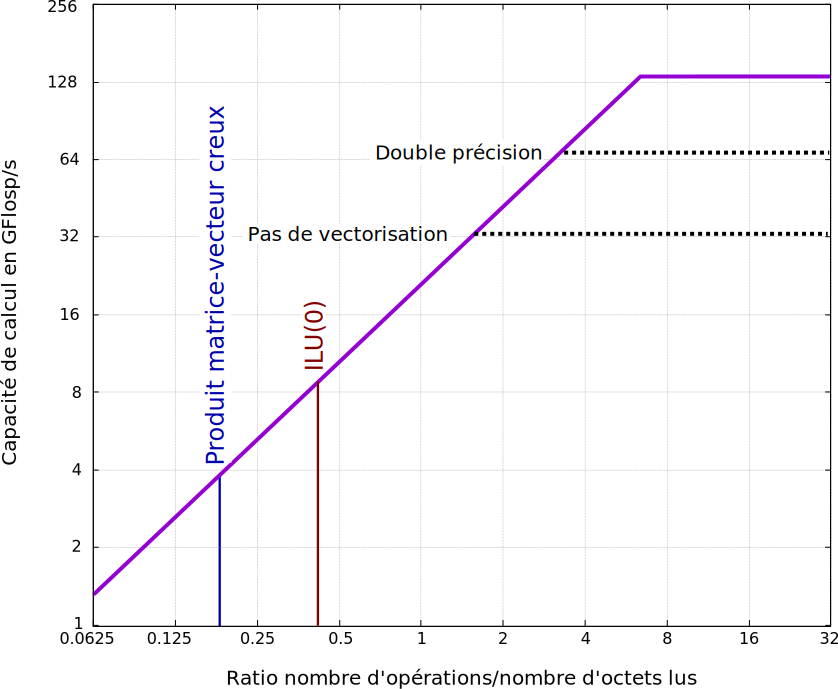
\includegraphics[width=0.8\textwidth]{roofline_rostand}
  \caption{Roofline model de Rostand. avec les différents produit matrice vecteur creux.}
  \label{fig:roofline_rostand}
\end{figure}
